\section{Examples of external-label disagreement}
\label{app:external_disagreements}

Figures~\ref{fig:disagree_gallery}--\ref{fig:disagree_gallery_3} show five examples per internal class with at least one mapped-label disagreement. Selection favours reference coverage and label diversity. Row labels give ensemble predictions; Cle, Hor, and Chi denote Clews, Horton, and Chilufya, with a dash for missing mapped labels. \(C\) denotes confidence. The two internal FRII classes remain separate in this inspection sample.

\begin{figure}[H]
\centering
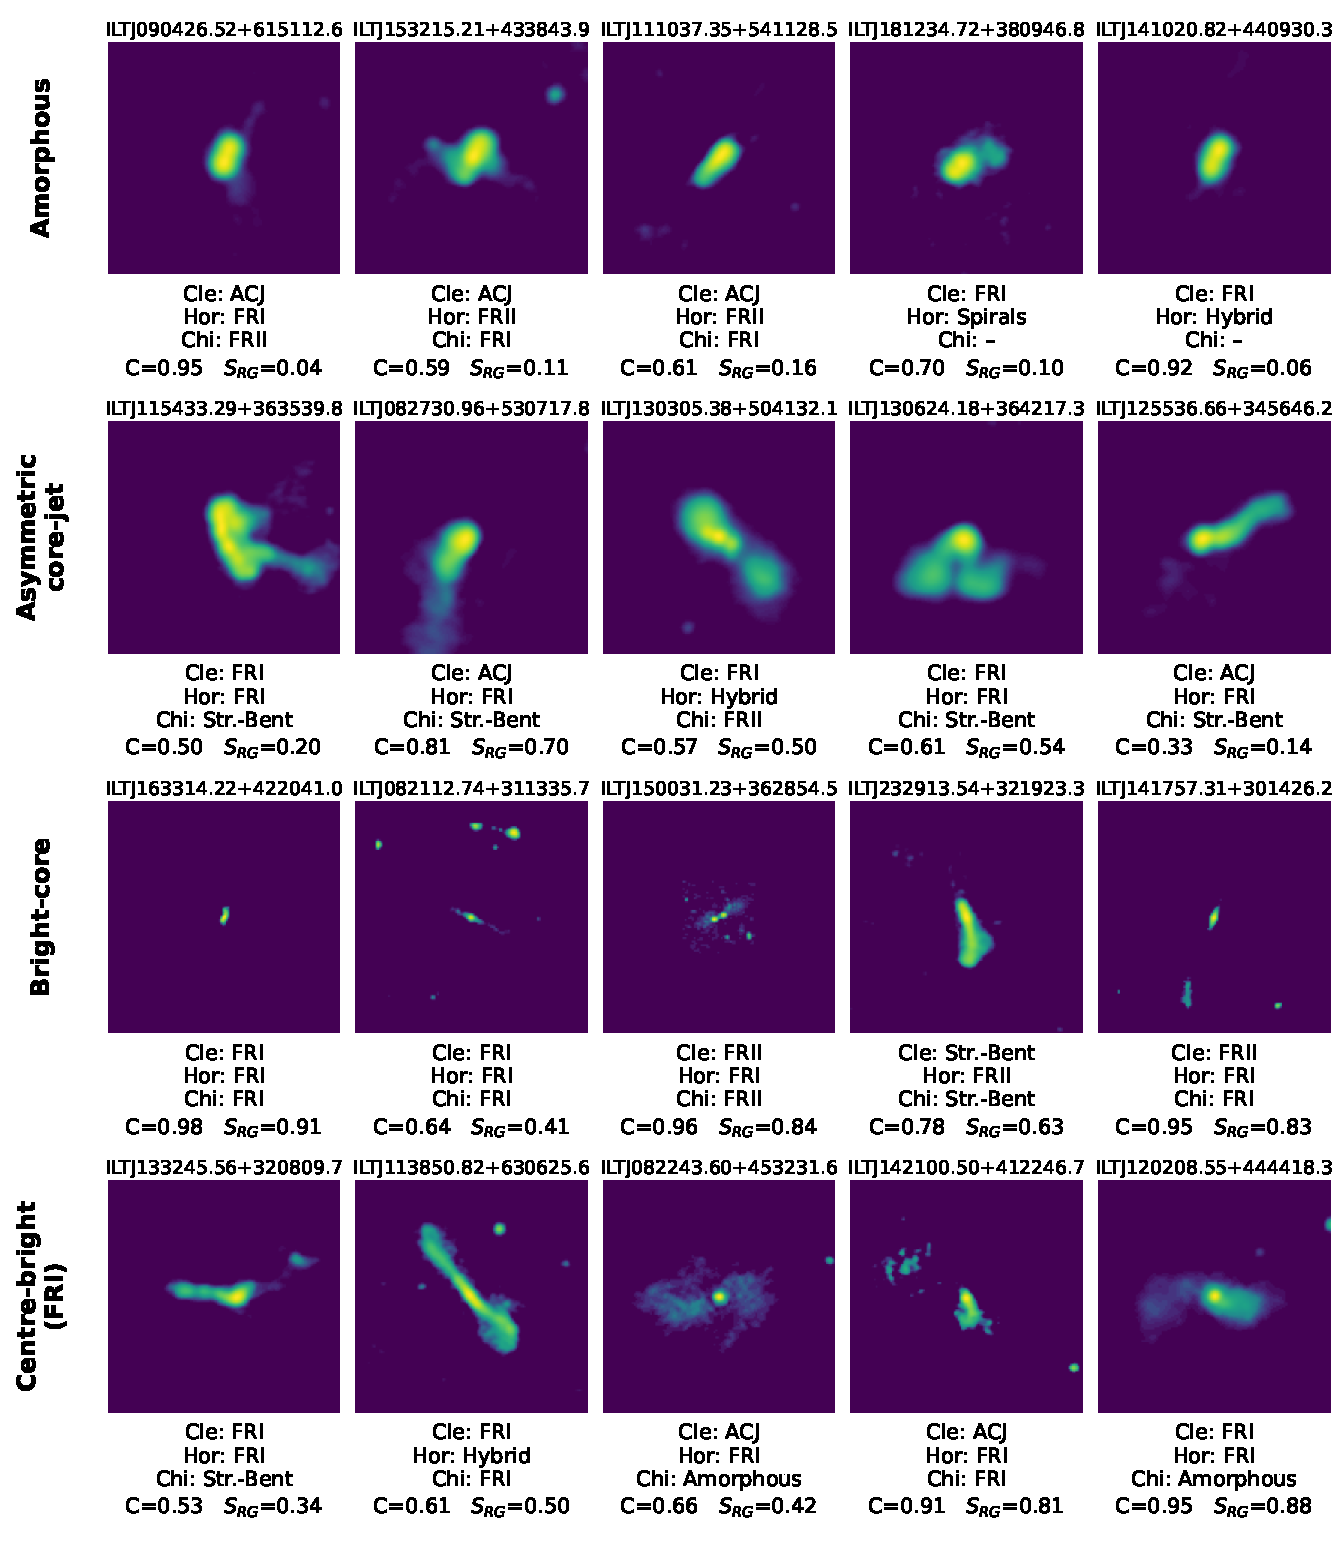
\includegraphics[width=\linewidth,height=0.73\textheight,keepaspectratio]{img/disagreement_gallery_1.pdf}
\caption[External disagreements: Amorphous, ACJ, Bright-core and FRI]{Five disagreement examples per class for Amorphous, ACJ, Bright-core, and FRI.}
\label{fig:disagree_gallery}
\end{figure}

\begin{figure}[p]
\centering
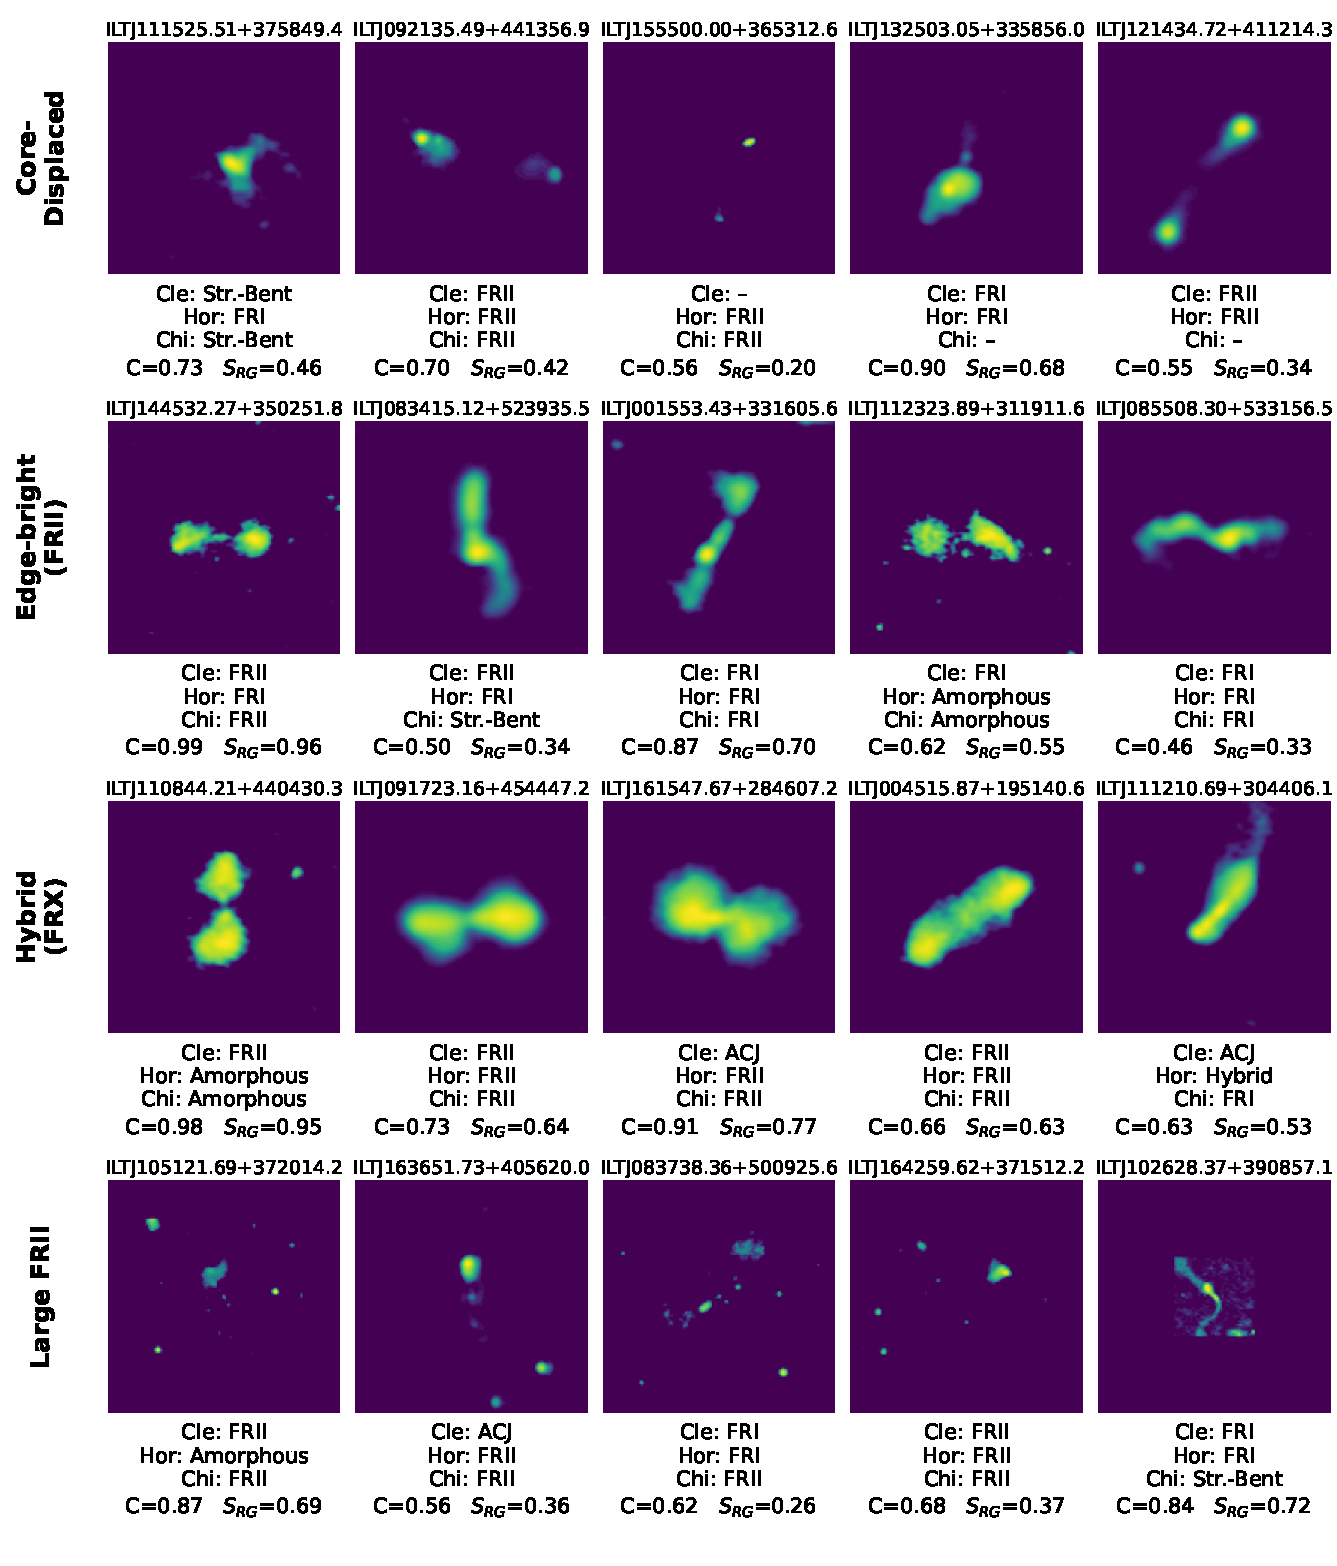
\includegraphics[width=\linewidth,height=0.87\textheight,keepaspectratio]{img/disagreement_gallery_2.pdf}
\caption[External disagreements: Core-Displaced, FRII, Hybrid and Large FRII]{Disagreement examples for Core-Displaced, FRII, Hybrid, and Large FRII. Annotations follow Figure~\ref{fig:disagree_gallery}.}
\label{fig:disagree_gallery_2}
\end{figure}

\begin{figure}[p]
\centering
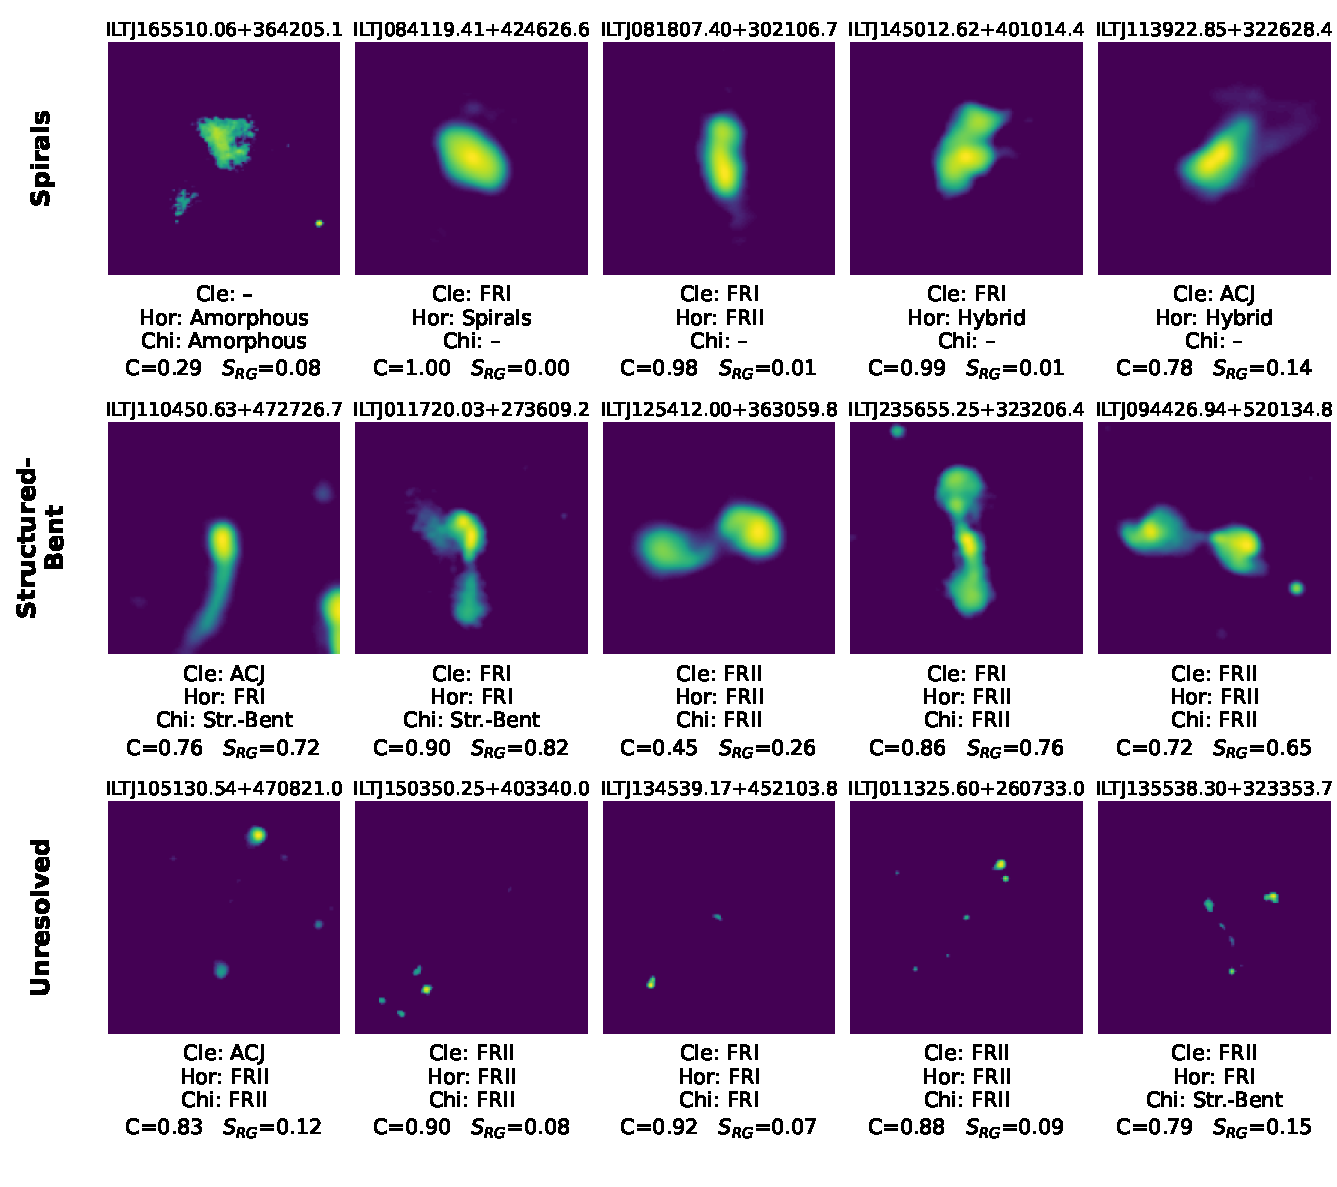
\includegraphics[width=\linewidth,height=0.87\textheight,keepaspectratio]{img/disagreement_gallery_3.pdf}
\caption[External disagreements: Spirals, Structured-Bent and Unresolved]{Disagreement examples for Spirals, Structured-Bent, and Unresolved. Annotations follow Figure~\ref{fig:disagree_gallery}.}
\label{fig:disagree_gallery_3}
\end{figure}
